\chapter{Projeto}

Assim como o EPOS, este trabalho baseia-se no conceito de especialização de classes C++. O sistema é estruturado fundamentalmente em duas camadas principais: a camada de mediadores de hardware,
composta por classes altamente especializadas e dedicadas à interação direta com os componentes físicos, e a camada de abstração, que utiliza os mediadores para implementar as
funcionalidades do sistema. Adicionalmente, há a camada de virtualização, que atua como ponte entre os sistemas virtualizados, os mediadores e as próprias abstrações da plataforma.

\begin{figure}[H]
\centering
\includegraphics[width=1\textwidth]{images/BlocksArchitecture.pdf}
\caption{Diagrama de Blocos das Classes do Projeto}\label{fig:blocks-architecture}
\end{figure}

Como ilustrado na Figura~\ref{fig:blocks-architecture}, o hipervisor desenvolvido neste trabalho — a exemplo de grande parte dos \gls{so} modernos — suporta dois tipos de aplicações:
aquelas executadas sobre máquinas virtuais e aquelas mapeadas para rodar no próprio hipervisor sem a necessidade de uma \gls{vm}. Essa abordagem é vantajosa em diversos cenários,
como na execução de tarefas em que a latência deve ser mínima e o desempenho máximo, além de cenários focados em verificação e auditoria de segurança.

\section{\Glspl{vm}}

\Glspl{vm} são a correspondência em software --- em nível de virtualização --- de máquinas físicas, podendo conter CPUs virtuais, memória e dispositivos periféricos.
Em correspondência com \glspl{so} modernos, \glspl{vm} funcionam de forma análoga a processos no projeto. Por definição, a criação de uma \gls{vm} deve receber uma porção
de memória alocada para si; esta será a região delimitada e autorizada a ser acessada pelo convidado. Além disso, para cada núcleo esperado pelo convidado, a \gls{vm} criará uma CPU virtual,
ficando também responsável por criar e gerenciar os dispositivos virtuais.

\begin{figure}[H]
\centering
\includegraphics[width=0.8\textwidth]{images/SimplifiedVirtualMachine.pdf}
\caption{Diagrama de Classes Simplificado de \glspl{vm}}\label{fig:simplified-virtual-machine}
\end{figure}

\section{CPU Virtual}

\Glspl{so} convidados não possuem conhecimento dos núcleos físicos do processador da plataforma.
Por isso, grande parte dos hipervisores, incluindo este, implementa o conceito de CPUs virtuais, que simulam na prática um núcleo físico do processador.
Dessa forma, para cada CPU de uma \gls{vm}, cria-se uma \textit{thread} encarregada de simular a execução de código do núcleo.

Além da execução de código, as CPUs virtuais também são responsáveis por redirecionar eventos às suas respectivas \glspl{vm}.
Como existe um mapeamento um para um entre \textit{threads} e CPUs virtuais, quando ocorre um evento, é possível verificar o ponteiro da CPU virtual em execução naquele instante e, por meio dela,
identificar a \gls{vm} correspondente.

\begin{figure}[H]
\centering
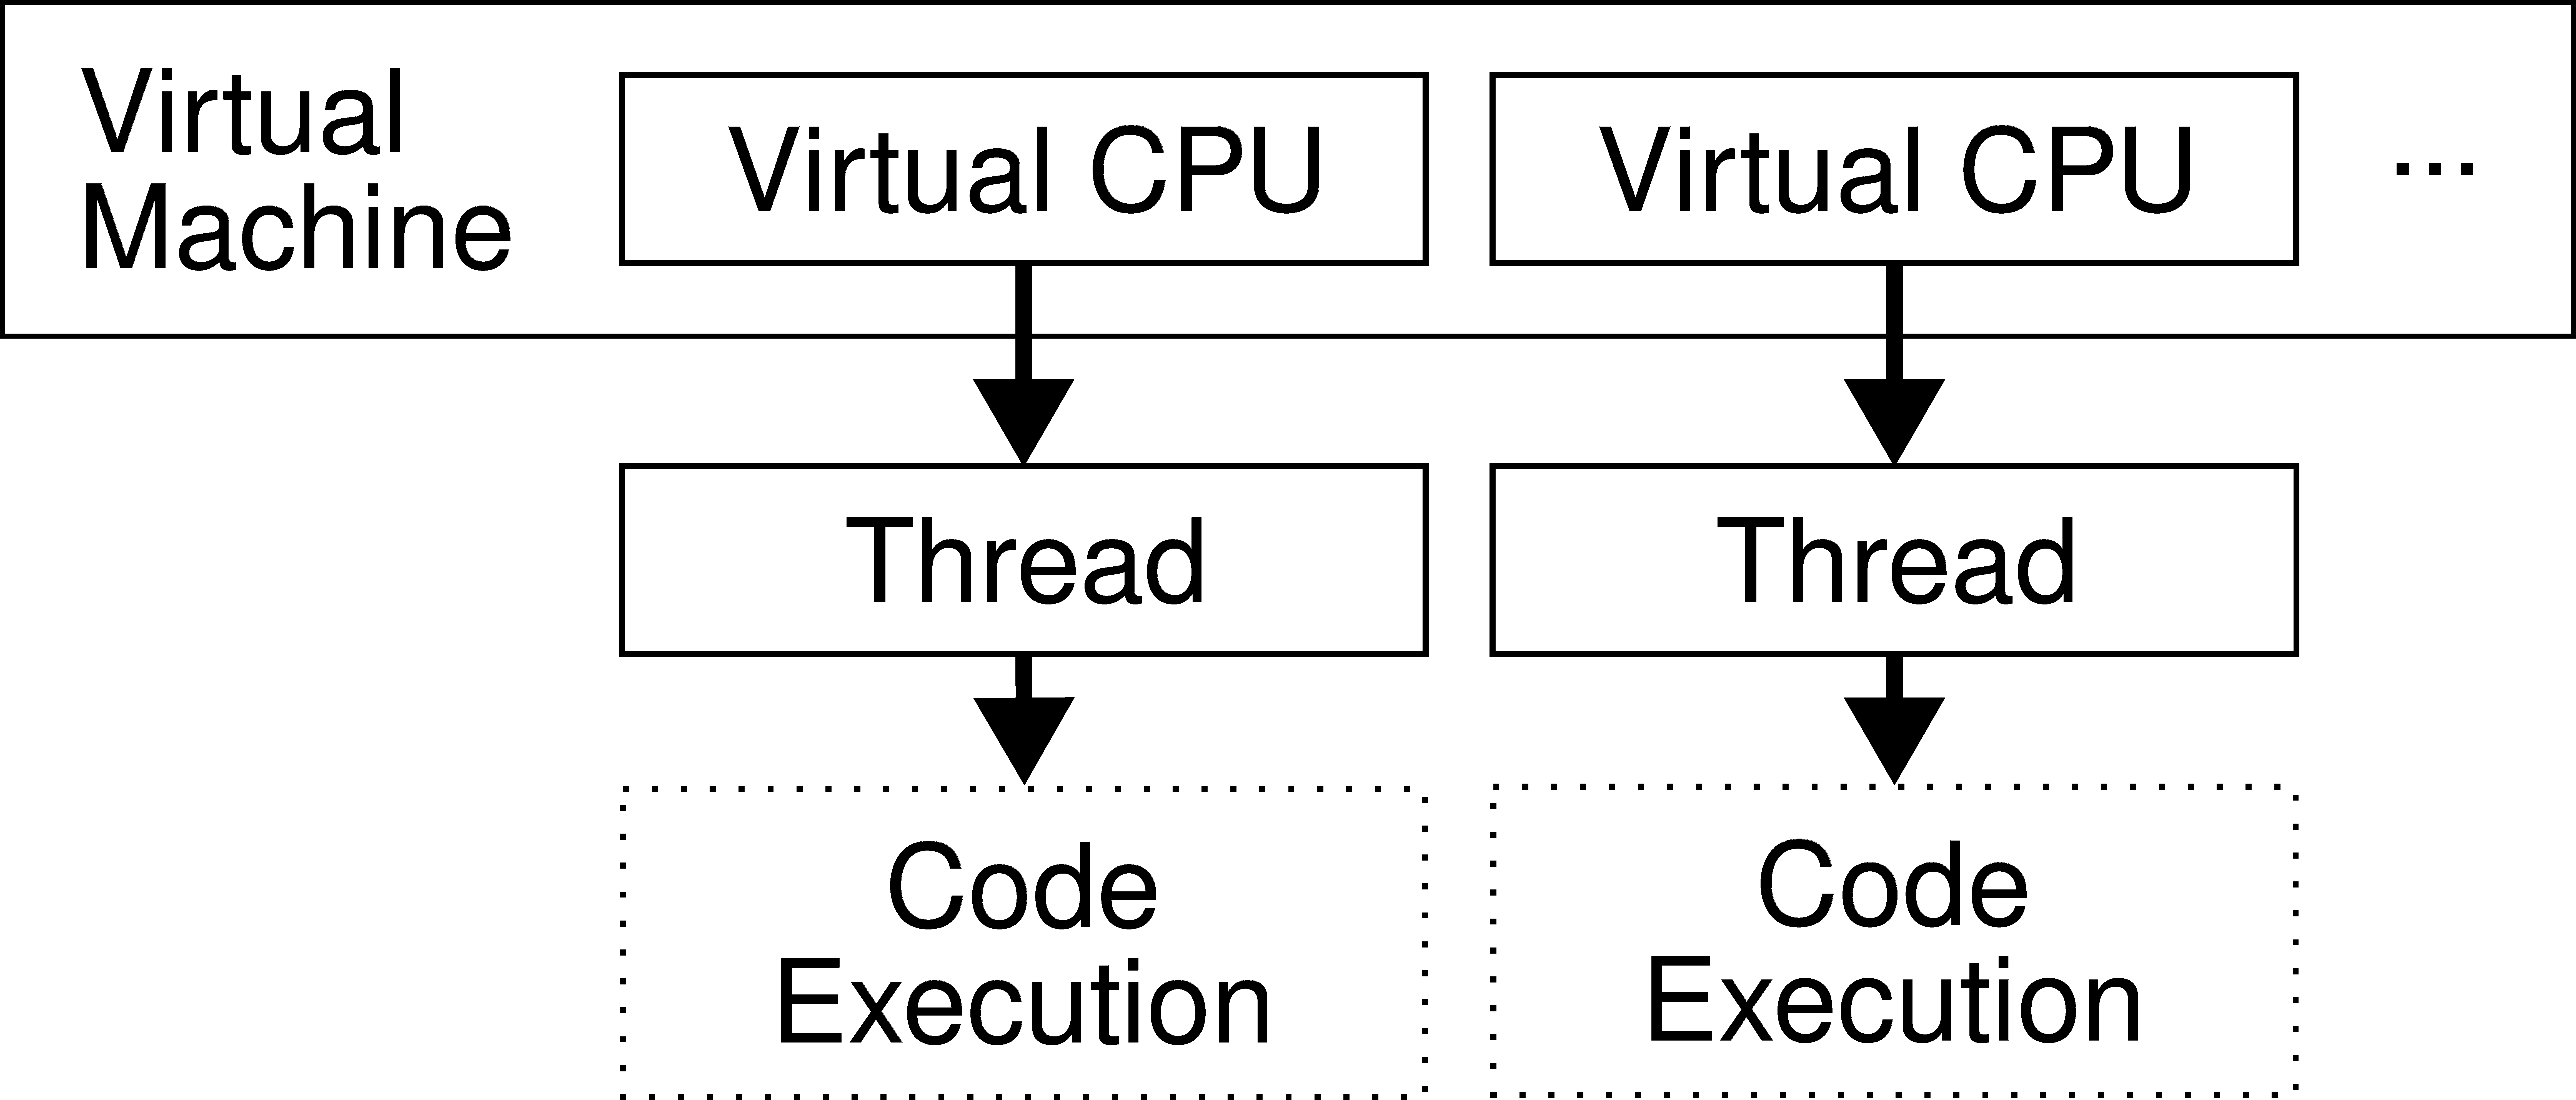
\includegraphics[width=0.6\textwidth]{images/VirtualCPUsToThreads.pdf}
\caption{Diagrama de Mapeamento de CPUs Virtuais Para Threads}\label{fig:virtual-cpus-to-threads}
\end{figure}

\section{Dispositivos Virtuais}

Dispositivos virtuais representam, para o \gls{so} convidado, dispositivos de hardware que podem ser utilizados para comunicação com a plataforma,
como temporizadores e dispositivos de \gls{io}. Eles abstraem os mecanismos de hardware utilizados pelo hipervisor, permitindo que o convidado interaja com esses
recursos sem acessar diretamente os dispositivos físicos.

\subsection{Comunicação: Convidado para Hardware}

A comunicação do \gls{so} convidado com o hardware é intermediada pelo hipervisor. As requisições do convidado podem chegar ao hipervisor tanto por meio da interceptação de operações
de acesso ao hardware quanto por chamadas direcionadas diretamente aos dispositivos virtuais. Em ambos os casos, o hipervisor encaminha a requisição ao objeto da \gls{vm} correspondente, que
identifica o dispositivo virtual responsável pela operação. O dispositivo virtual, por sua vez, traduz e encaminha a requisição ao mediador de hardware correspondente,
conforme ilustrado na Figura~\ref{fig:diagram-hosted-to-hardware}.

\begin{figure}[H]
\centering
\includegraphics[width=1\textwidth]{images/VirtualDeviceToHardware.pdf}
\caption{Diagrama do Fluxo de Comunicação: Convidado para Hardware}\label{fig:diagram-hosted-to-hardware}
\end{figure}

\subsection{Comunicação: Hardware para Convidado}

O fluxo de notificação de um evento de hardware para o \gls{so} convidado é ilustrado na Figura~\ref{fig:diagram-hardware-to-hosted}.
Esse mecanismo baseia-se no padrão de projeto \textit{Observer}, no qual cada mediador de hardware atua como um elemento observável e cada dispositivo virtual funciona como um observador.

Quando ocorre um evento no mediador de hardware, este notifica seus observadores cadastrados, propagando a sinalização até que o dispositivo virtual correspondente
processe a informação e a entregue ao domínio do SO convidado.

\begin{figure}[H]
\centering
\includegraphics[width=1\textwidth]{images/HardwareToVirtualDevice.pdf}
\caption{Diagrama do Fluxo de Comunicação: Hardware para Convidado}\label{fig:diagram-hardware-to-hosted}
\end{figure}

\section{Integração}

A integração dos componentes, conforme mencionado anteriormente, ocorre por meio da agregação de todos os recursos de que uma \gls{vm} necessita em sua própria classe.
Além disso, cada mediador virtual possui um mapeamento específico para um mediador real, como ilustrado na Figura~\ref{fig:virtual-to-real}.

\begin{figure}[H]
\centering
\includegraphics[width=0.6\textwidth]{images/VirtualToReal.pdf}
\caption{Diagrama de Mapeamento de Componentes Virtuais para Reais}\label{fig:virtual-to-real}
\end{figure}

Formalizando essa estrutura, a interface mínima que a camada de virtualização fornece é apresentada na Figura~\ref{fig:virtualization-framework-uml}.

\begin{figure}[H]
\centering
\includegraphics[width=0.8\textwidth]{images/VirtualizationFrameworkUML.pdf}
\caption{Diagrama de Classes Relacionadas ao Processo de Virtualização}\label{fig:virtualization-framework-uml}
\end{figure}

